%!TEX root = ../thesis.tex

\chapter{Related Work}
\label{chapter_related_work}

While existing practices require tutorial authors to create instructions manually, HCI and Computer Graphics communities have introduced novel technologies for authoring tutorials, including automatic generation methods and interactive editing tools.
%
In this chapter, I survey state-of-the-art techniques for generating instructions for both software applications (Section \ref{related_software}) and physical tasks (Section \ref{related_physical}).
%
Furthermore, existing instructions are mainly offered in the forms of conventional media, such as static tutorials (print-outs or web) or videos. With software systems, \keyword{interactive tutorials} have been introduced for learners to interactively review instructional content. I will discuss various forms of such kind of instructions by prior research, which leads to a discussion on the remaining gaps in tool support for creating and navigating instructional content.
%
Finally, in Section \ref{related_videos}, I review the methods of video analysis and playback.

% -------------------------------------------

\section{Instructions for Software Applications}
\label{related_software}

\subsection{Input Event Visualization}

% real-time
Studies have shown that visualizing input events in real-time during operations can provide better learnability of applications~\cite{Dixon:2010fb}. Events can range from low-level, application agnostic input device events (e.g., mouse actions, cursor movements, or keyboard strokes) to higher level, application-dependent information (e.g., menu selections or UI component changes).
%
Commercial tools such as Mouseposé\footnote{\url{http://www.boinx.com/mousepose}} and ScreenFlow\footnote{\url{http://www.telestream.net/screenflow}} visualize mouse events and keystrokes with special effects, e.g., drawing a circle around a mouse cursor (see Figure~\ref{fig:related_realtime} top). These tools capture input information (e.g., mouse position and event type) and render visualization on top of the screen activities. This approach is commonly adopted by online video tutorial authors. However, it does not consider application context, which can be difficult for learners to follow specific instructions at a semantic level, such as observing a complete text field or drop-down menu option.
% Some further enable video editing techniques, including zooming in/out  and panning.

To visualization UI components (e.g., a checkbox, button, or editable text field), Dixon \ea{}'s Prefab~\cite{Dixon:2010fb,Dixon:2011:CHP:1978942.1979086} provides pixel-based enhancements in real-time by detecting target features, such as region corners. This semantic understanding of GUI enables component-based highlighting effects, such as afterglows~\cite{Baudisch:2006:PET:1166253.1166280} that visualize user operations (see Figure~\ref{fig:related_realtime} bottom left) and Bubble Cursor~\cite{Grossman:2005:BCE:1054972.1055012}, a target-aware pointing technique that suggests the nearest target (see Figure~\ref{fig:related_realtime} bottom right).

\begin{figure*}[t!]
  \centering
  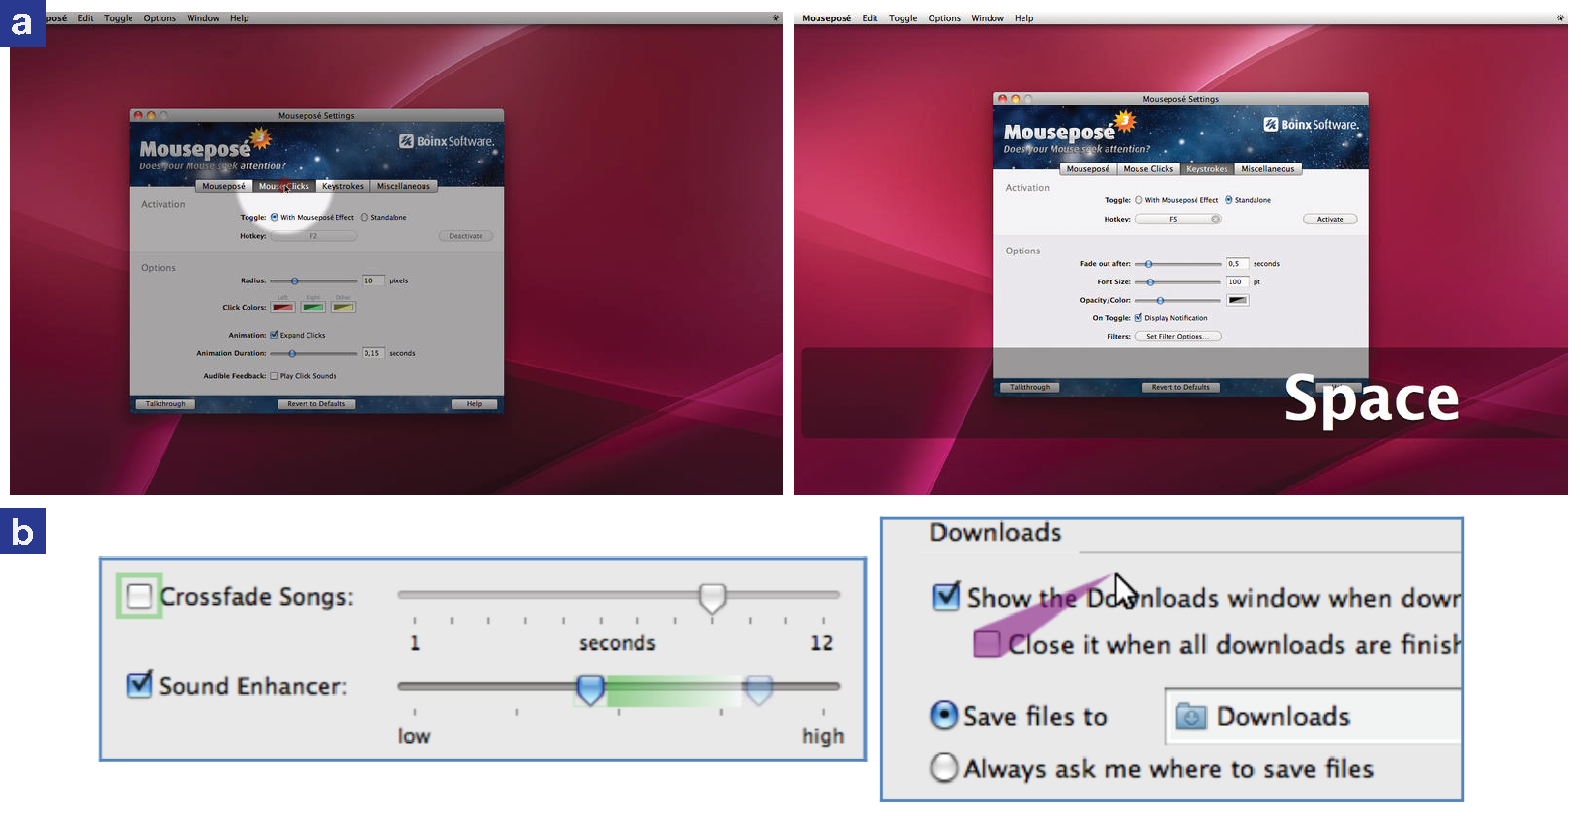
\includegraphics[width=0.7\textwidth]{\background/fig/realtime/realtime}
  \caption{Real-time visual enhancements on GUI applications: (top) Mouseposé highlights mouse cursors or keyboard input; (bottom) Prefab~\cite{Dixon:2010fb} performs reverse engineering to identify UI components and enable real-time visualizations during author operations, such as afterglow~\cite{Baudisch:2006:PET:1166253.1166280} and target-aware~\cite{Grossman:2005:BCE:1054972.1055012} effects.}
  \label{fig:related_realtime}
\end{figure*}

\begin{figure*}[t!]
  \centering
  \includegraphics[width=0.6\textwidth]{\background/fig/software_viz/Nakamura_and_Igarashi}
  \includegraphics[width=\textwidth]{\background/fig/software_viz/Grabler}
  \caption{Example screenshots that visualize mouse operations are automatically rendered, including (top) mouse move, drag, click, and wheel (a-d) by Nakamura and Igarashi~\cite{Nakamura:2008:ASV:1449715.1449721} and (bottom) application-specific operations (a-b), parameters (c-f), and manipulations (g-h) by Grabler \ea{}~\cite{Grabler:2009jj}.}
  \label{fig:related_events}
\end{figure*}

% in screenshots
The above methods enable real-time visualization of input events when operating an application, which are useful for following a video tutorial. But for screenshot images in a static tutorial, visualizing input actions with motion arrows is a common technique that provides a sense of direction and start and end positions, such as dragging a slider to the right.
%
Researchers have investigated automatic approaches that capture and visualize these types of events in representative screenshots from author demonstrations. Nakamura and Igarashi~\cite{Nakamura:2008:ASV:1449715.1449721} proposed a capturing and rendering system independent to GUI applications. Their system logs mouse events of a software demo process, including mouse moving, dragging, and clicking. Operations are rendered as markers and arrows on screenshot images to present the linear event history (see Figure~\ref{fig:related_events} top).
%
Grabler \ea{}'s approach~\cite{Grabler:2009jj} further annotates screenshots with bounding boxes and call-outs, which help learners identify parameters and options of software functionalities (see Figure~\ref{fig:related_events} bottom).

% summary
Our systems adopt some of these successful techniques to enhance instructions. By capturing event information at both input and application levels, we visualize author operations based on different playback modes.
%
During video playback, MixT shows mouse trails and actions, and DemoWiz overlays glyphs and arrows to guide viewers from the current input action to the next.
%
To generate static, step-by-step tutorials, MixT renders screenshot images with mouse visualizations, such as highlighting a drop-down menu.

% -------------------

\subsection{Workflow Capturing and Tutorials}
In addition to visualizing input events, it is important to present the entire workflow in a tutorial and provide concise instructions.
%
Grabler \ea{}'s system~\cite{Grabler:2009jj} generates step-by-step tutorials from an author demonstration (see Figure~\ref{fig:related_static}). Designed for instructing image manipulation software, it includes textual description from templates, such as \iquote{Select the \textbf{path tool} from the \textbf{toolbar} to \textbf{create and edit paths}.} The generated text and annotated images of operations are presented as a static tutorial to describe the workflow. Their work is available as a Photoshop plug-in\footnote{Adobe labs. Tutorial Builder. \url{http://labs.adobe.com/technologies/tutorialbuilder/}}.
% analyzes the application context, including facial features and outdoor scenes in manipulated images.
%
Such demonstration-based approaches for generating instructions have been applied to applications that involve more complicated manipulations or gestures, including 3D mesh construction~\cite{Denning:2011fy} and mobile applications~\cite{Wang:2014:EAC:2556288.2557407}.
%
Beyond logging events from recording a user demonstration, researchers have shown that workflows and software content can be captured automatically using computer vision from analyzing desktop regions~\cite{Yeh:2009dh,Chang:2011vd} and existing screencast videos~\cite{Banovic:2012kd}.

\begin{figure*}[t!]
  \centering
  \includegraphics[width=0.8\textwidth]{\background/fig/related_static/grabler}
  \caption{Example static tutorial automatically generated by Grabler \ea{}'s system~\cite{Grabler:2009jj}.}
  \label{fig:related_static}
\end{figure*}

To compare effects of individual operations in a workflow, showing a list of ``before'' and ``after'' thumbnails, video clips, and event timeline can be effective \cite{Grossman:2010jz}, especially for image manipulation tasks (see Figure~\ref{fig:related_comparison} left).
%
When there are multiple workflows that all create similar results, a union graph and presenting two instructional documents side-by-side are useful for comparing operations \cite{Kong:2012:DTR:2207676.2208549} (see Figure~\ref{fig:related_comparison} right).

\begin{figure*}[t!]
  \centering
  \includegraphics[width=0.4\textwidth]{\background/fig/software_viz/Grossman}
  \includegraphics[width=0.55\textwidth]{\background/fig/software_viz/Kong}
  \caption{Instructional systems that help learners compare effects and similar tutorials using: (left) before and after images (a) and event timeline (b) by Grossman \ea{}~\cite{Grossman:2010jz} and (right) operation union graph by Kong \ea{}~\cite{Kong:2012:DTR:2207676.2208549}.}
  \label{fig:related_comparison}
\end{figure*}

% summary
These systems provided insights on 1) automatic generation methods of step-by-step tutorials and 2) a variety of presentations of showing workflows for different purposes. Our MixT system is built based on the Photoshop plug-in (Tutorial Builder) to acquire a step-by-step document with text descriptions. We enhance the static tutorial format by embedding instructional video clips for each step that can be interactively reviewed.

This paradigm opens a design space to create new tutorial formats that can be interactively reviewed. In recent years, researchers have shown that learners using responsive video tutorials~\cite{Nguyen:2015:MST:2702123.2702209} and learning-by-doing activities~\cite{Kwon:2016:CEO:2858036.2858101} performed better in learning than using static or video tutorials.

% -------------------

\subsection{In-Application Support}

The above methods introduce innovative ways for learners to review workflows and instructions. However, reviewing these materials is often separated from operating a software application. Learners might have to switch between the main application they are using and a separate set of instructions, which could introduce a gap of evaluation (\iquote{Am I doing this right as the instructions explain?}) and a gap of execution (\iquote{How do I perform the action that the instructions describe?}).
%
Researchers have proposed another approach to provide ``in-application'' assistance, often in real-time, in a specific application context.

There has been a considerable amount of research devoted to offering interactive help to support learners comprehend the functionalities while operating an application.
%
Crystal~\cite{Myers:2006:AWW:1124772.1124832} enables software users ask questions about ``why'' something did or did not occur in an application.
%
Video snippets can be embedded in application tooltips to explain specific functionalities~\cite{Grossman:2010wr}, which were shown to be seven times more effective than conventional tooltips for completing unfamiliar tasks.

Interactive, step-by-step instructions can be integrated in several forms:
%
To help software user identify the correct UI components, tutorials can be shown via translucent colored ``stencils,'' which visually direct user's attention directly in an application~\cite{Kelleher:2005:STD:1054972.1055047}.
%
By tracking user's current operations, tutorials can be embedded in an application to provide instant feedback such as a check-mark or a percentage match~\cite{Fernquist:2011:SRE:2047196.2047245}, automatically replayed to provide the corresponding video instructions~\cite{Pongnumkul:2011ju}, or be shown as ambient help~\cite{Matejka:2011:AH:1978942.1979349}.
%
Instructions can be captured from demonstration as ``scripts'' for step-by-step navigation~\cite{Bergman:2005:DocWizards}. Having more user controls~\cite{Lieberman:2014:SML:2557500.2557543} or being enhanced with game elements~\cite{Li:2014:CGM:2556288.2556954, Dontcheva:2014:CCL:2556288.2557217} can further engage users in learning.

Last but not least, as tutorials are built for a broader community with a set of authors and learners, content can be dynamically updated within a community based on user contribution~\cite{Lafreniere:2013ff,Matejka:2009:CCR:1622176.1622214, Bunt:2014:TPI:2556288.2557118}.

Although our work focuses on authoring tools to create novel tutorial format designs, we see opportunities of combining our approaches with in-application guidance. For example, a video clip from a MixT tutorial can be automatically replayed when a system detects a slowdown of a learner's progress on a specific step. However, we do not claim contribution in this direction.

% These projects show how effective instructional representations can assist learners in learning or executing tasks. Our goal is to further study new formats that incorporate advantages of several formats of multimedia, including images, text, and videos, and in turn enhancing the learning experience for a variety of tasks.

% * define ``automatic''
% Note: MixT tutorials are automatically rendered from manual demonstration, not automatically generated.

% To provide real-time assistance, it is important to recognize the user activities during a task performance. Several domains have been widely studied, including software operations, scene recognition, and object tracking in a physical world.

% -------------------------------------------

\section{Instructions for Physical Activities}
\label{related_physical}

The above approaches of tracking user behavior to automate tutorial authoring opens the door to interactive tutorials that can respond to user progress. However, tracking user behavior in the physical world, rather than in software, remains a challenge.
%
To record activities and provide responsive feedback, a computer system needs to understand user operations and objects in real-time. %Ideally, activities should be automatically tracked without human labeling.
%
Computer vision techniques can track specific physical targets shown in a video, including objects (e.g., a fast-moving Ping-Pong ball~\cite{Okumura:2011tr} or regions in pre-defined spaces~\cite{Ranjan:2007}), humans (e.g., faces, hands~\cite{taylor-siggraph2016,Ranjan:2008}, and user movements~\cite{Wilson:2012fb}), and a combination (e.g., a player throwing a basketball~\cite{dou-siggraph2016}).
%
% These methods usually require an expert defining heuristics of space regions or movement classifications ahead of time for the tracking program.
% Thanks to the advance of technology, camera sensors such as Kinect have become widely available to track activities for block assembly~\cite{Gupta:2012ku} and dance~\cite{Anderson:2013:YEM:2501988.2502045}.

\subsection{Generating Instructions for Real-World Tasks}
Researchers have investigated tools for automatically generating visual instructions for physical tasks~\cite{feiner:1985:AEA:1299975.1300548,Seligmann:1991:AGI:127719.122732}. Workflows can be captured and created for furniture \cite{agrawala2003designing} or block assembly tasks \cite{Gupta:2012ku}.
%
If video content is difficult to be extracted, crowdsourcing algorithms have been introduced to structure step-by-step videos by online workers~\cite{Kim:2014:CSI:2611222.2556986}.
%
% New devices to support authors capturing multi-media materials, such as a turntable~\cite{Tseng:2015:SPT:2771839.2771869}
% documentation \cite{Tseng:2016:makeology}

\subsection{Interactive Guidance}
To provide responsive instructions, a computer system needs to understand user operations in real-time. Ideally, activities should be automatically tracked without human labeling.
%
Computer vision techniques can track specific physical targets, including hands \cite{Ranjan:2008}, user movements \cite{Wilson:2012fb}, fast-moving objects (e.g., a Ping-Pong ball) \cite{Okumura:2011tr}, or regions in pre-defined spaces \cite{Ranjan:2007}.
%
These methods usually require an expert defining heuristics of space regions or movement classifications ahead of time for the tracking program.
%
Thanks to the advance of technology, camera sensors such as Kinect have become widely available to track activities for block assembly~\cite{Gupta:2012ku} and dance~\cite{Anderson:2013:YEM:2501988.2502045}.

Real-time guidance is often shown via an external display, placed next to the working area~\cite{Gupta:2012ku}. To better blend the information into activities, Knibbe~\ea{} designed a display-embedded table as a physical workspace that monitors, records, and assists users~\cite{Knibbe:2015:SMI:2817721.2817741}.
%
Alternatively, information can be overlaid on top of the work area using augmented reality, usually through a head-mounted display. Such systems can provide visual highlights for machine maintenance~\cite{Henderson:2011ff}, or interactive remote tutoring for repair tasks~\cite{Gurevich:2012ko}.
%
Another method is to overlay guidance on an augmented mirror for tasks such as dance movements~\cite{Anderson:2013:YEM:2501988.2502045}.

for Frisbee players~\cite{Solomon:2014:UTI:2540930.2540965}

% Lovell and Buechley use electrical sensing with conductive thread for a sewing tutorial~\cite{Lovell:2010tl}.

% I aim to propose a new approach that gives users flexibility in a home environment, and provides interactive control. If activity recognition is not possible, my approach includes users in the loop to annotate high-level information in order to create high-quality results.

% -------------------------------------------

\section{Working with Videos}
\label{related_videos}

\subsection{Capture}
Several research and commercial systems guide users at capture time to yield higher-quality videos. Such systems often employ templates to help users capture sequences of distinct shots (e.g., Snapguide\footnote{\url{http://snapguide.com/}}) or suggest framing of the subject or camera view as in NudgeCam~\cite{Carter:2010}. Computer vision algorithms, like face tracking, can be used to offer real-time feedback during such directed actions~\cite{Davis:2003cu,Heer:2004ba,Carter:2010}. Instead of relying on templates, shot suggestions can also be bootstrapped through user dialogs~\cite{Adams:2005}.

\subsection{Annotation}
Researchers have investigated how to provide interactions that enable efficient, fluid annotation of video data, from the early EVA system~\cite{Mackay:1989} to more recent interfaces like VideoTater that leverage pen input~\cite{Diakopoulos:2006vt}.

\subsection{Editing}
Frame-based editing of video is very time-intensive, as it forces users to operate at a very low level of detail. Editors can leverage metadata, such as transcripts~\cite{Berthouzoz:2012,Pavel:2014:VDB:2642918.2647400} and shot boundaries~\cite{Casares:2002dx}, to give users higher-level editing operations at the shot level rather than the frame level.
In specific video domains like interview videos, transcripts can help users place cuts and transitions~\cite{Berthouzoz:2012}.
%
Computer vision techniques can automate certain effects, such as creating cinemagraphs~\cite{Bai:2012, Joshi:2012}, automatically-edited lecture videos~\cite{Heck:2007}, zoomable tapestries~\cite{Barnes:2010} and synopses~\cite{Pritch:2009vl}, or stabilizing shaky amateur videos~\cite{Liu:2011}. When analyzing video is a matter of subjective taste, identifying salient frames can also be outsourced to crowd workers~\cite{Bernstein:2011uj}.

live authoring through compositing and editing of streaming video~\cite{Freeman:2014:LLA:2611105.2557304}

\subsection{Navigating}
Videos can be navigated at the content level beyond log events, such as visualizing subject movements in a storyboard design \cite{goldman2006schematic} and enabling direct manipulation of a target in 2D \cite{Dragicevic:2008:VBD:1357054.1357096,Goldman:2008:VOA:1449715.1449719,Karrer:2008:DDM:1357054.1357097} or 3D \cite{Nguyen:2013:DMV:2470654.2466150}. These techniques help viewers understand content flow and playback videos, and have been applied to screencast videos \cite{Denoue:2013:RDM:2451176.2451190}. It is also possible to automate video control based on user actions for scenarios such as operating software applications~\cite{Pongnumkul:2011ju} and block assembling tasks \cite{Gupta:2012ku}. Such novel forms of video navigation inspired us to explore new visual designs for revealing the video content that support live presentations.

lecture videos~\cite{Tang:2006:DIU:1111449.1111523}

Visualization of personal history for video navigation~\cite{Al-Hajri:2014:VPH:2611105.2557106}

% In contrast to these systems, we do not require the author to manipulate the camera or system during capture. Many leisure activities, such as home repair or cooking, require use of both hands or involve getting one's hands dirty, so camera manipulation is not possible. We use vision techniques for automatic recording and editing. It differs from previous approaches in its focus on particular application domains -- software and physical demonstrations. By focusing on specific domains, we can make assumptions about the structure of the input and output video, such as the fact that there is a linear set of steps or movements, and offer user interfaces and algorithms that make it easier to create high quality instructions.
